25. $(|y|-3)(y+|x|-1)=0\Leftrightarrow \left[\begin{array}{l} |y|-3=0,\\ y+|x|-1=0.\end{array}\right.\Leftrightarrow\left[\begin{array}{l} y=3,\\ y=-3,\\ y=1-|x|.\end{array}\right.$
$$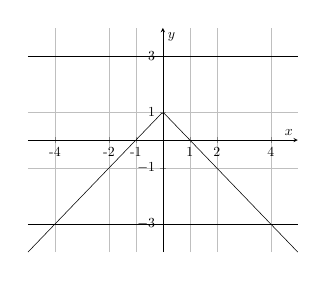
\begin{tikzpicture}[scale=0.5]
\begin{axis}[
    axis lines = middle,
    grid=major,
    legend pos={south west},
    xlabel = {$x$},
    %xlabel style={below right},
    ylabel = {$y$},
    ymin=-4,
    ymax=4,
    xtick={-4, -2,-1,1, 2,4},
    xticklabels={-4, -2,-1,1, 2, 4},
    ytick={1,-1,-3,3},
     %yticklabels={-5,-4,$ $,$-\frac{3}{2}$,6},
                  ]
	\addplot[domain=-5:5, samples=100, color=black] {3};
    \addplot[domain=-5:5, samples=100, color=black] {-3};
    \addplot[domain=-5:5, samples=100, color=black] {1-abs(x)};
	%\addlegendentry{$\text{Рис. 1}$};
\end{axis}
%\draw (3.7,3.05) circle (2pt);
\end{tikzpicture}$$
